\documentclass[11pt, titlepage]{article}
\usepackage[utf8]{inputenc}     % UTF-8 encoding
\usepackage[T1]{fontenc}
\usepackage{lmodern}
\usepackage[
    a4paper,
    outer=2cm,
    inner=2cm,
    top=2.5cm,
    bottom=2.5cm
]{geometry}
\usepackage{plain,graphicx,subcaption,svg}
\usepackage{wrapfig}            % Text and figures side by side
\usepackage{csquotes}           % Better quotes (\enquote{...}, \MakeOuterQuote{"} to make " work as a correct quote)
\usepackage{microtype}          % Better typography
\usepackage{enumitem}           % Customizable lists
\usepackage{tabularray}         % Better tables
\usepackage{caption}
\usepackage{fancyhdr}
\usepackage[english]{babel}

\usepackage{amsmath,amssymb}
\usepackage{booktabs}
\usepackage{xcolor}
\usepackage{listings}
\usepackage{algorithm}
\usepackage{algpseudocode}
\usepackage{pgfplots}
\pgfplotsset{compat=1.17}

% hyperref, then cleveref, must come last (needs amsmath before)
\usepackage[hidelinks]{hyperref}             % Clickable links without ugly boxes
\usepackage[capitalize,noabbrev]{cleveref}   % Smarter cross-referencing

% some helpers
\newcommand{\TODO}[1]{\textcolor{red}{[TODO: #1]}}
\newcommand{\kth}{$k$-th smallest}

\begin{document}
\thispagestyle{empty}
\begin{center}
    \begin{figure}[h!]
        \centering
        
\includegraphics[width=.6\textwidth]{images/unitn.png}
    \end{figure}
    \vspace{6 cm}
    \Huge\textsc{High Performance Computing for Data Science\\}
    \vspace{0.5 cm}
    \huge{Project Report\\}
    \vspace{3.5 cm}
    \Large{Lorenzo Cortese 273920\\ Alessandro Marostica 265433}
\end{center}
\clearpage

\begin{abstract}
  \TODO{Ce lo mettiamo? Secondo me no}
\end{abstract}

\tableofcontents
\newpage

% Introduzione, spiegazione problema and shit
\section{Introduction}\label{sec:intro}
Given an unsorted array $A$ of $n$ integers and an index $k$, the \emph{selection problem} asks for the element of rank $k$, i.e.\ the value that would be at position $k$ if $A$ were sorted. $k=0$ is the minimum and $k=\lfloor n/2\rfloor$ the median. \TODO{specificare convenzione (0-based qua), il formato dell'input (file binario: \texttt{int64} header $n$ seguito da $n$ \texttt{int32} valori in little endian), e e dimensioni target.}

\subsection{Applications and motivation}
\TODO{filtri mediani, statistiche di ordine, quantili nei database, punti di divisione in sorting parallelo, ...}

\subsection{Sequential algorithms}
\paragraph{Sort and index.} $\Theta(n\log n)$; simple but does more work than needed.

\paragraph{Quickselect (Hoare).}
Partition around a pivot, recurse only on the side containing rank $k$. Expected $\Theta(n)$, worst case $\Theta(n^2)$.
\TODO{Maybe pseudocode a un piccolo esempio?}

\paragraph{Median of Medians (Blum et al.).}
Choosing as pivot the median of the medians of blocks of constant size guarantees that a constant fraction of the elements is discarded at every step, giving worst-case $\Theta(n)$.
\TODO{derivazione della ricorrenza $T(n)\le T(n/b + \cdot)+T(\alpha n)+O(n)$ e dello shrink factor la block size}

\begin{algorithm}[t]
  \caption{Sequential selection (quickselect, 0-based rank $k$)}\label{alg:qselect}
  \begin{algorithmic}[1]
    \Function{Select}{$A,k$}
    \State choose a pivot $x$ \Comment{random, median of 3, or median of medians}
    \State partition $A$ into $L=\{a<x\}$, $E=\{a=x\}$, $G=\{a>x\}$
    \If{$k<|L|$} \Return \Call{Select}{$L,k$}
    \ElsIf{$k<|L|+|E|$} \Return $x$
    \Else{} \Return \Call{Select}{$G,k-|L|-|E|$}
    \EndIf
    \EndFunction
  \end{algorithmic}
\end{algorithm}

\subsection{Complexity Summary}
\begin{table}[h]
  \centering
  \begin{tabular}{lll}
    \toprule
    Algorithm & Expected & Worst case\\
    \midrule
    Sort + index & $\Theta(n\log n)$ & $\Theta(n\log n)$\\
    Quickselect & $\Theta(n)$ & $\Theta(n^2)$\\
    Median of medians & $\Theta(n)$ & $\Theta(n)$\\
    \bottomrule	
  \end{tabular}
  \caption{Sequential selection algorithms.}
\end{table}

\subsection{Report organization}
\TODO{anche questa, la mettiamo o no?}

% design parallelo
\section{Parallel design}\label{sec:design}

\subsection{Sources of parallelism}
Where the sequential algorithm can be parallelized and where it cannot:
\begin{itemize}
\item \textbf{Partitioning} is a linear scan with independent iterations (each element is compared to the pivot): parallel by splitting the array; the counts $|L|,|E|,|G|$ are combined with a reduction.
\item \textbf{Pivot selection}: the medians of the blocks are independent (\texttt{pardo} in the lecture notes); only the final combination of the candidates is sequential and small.
\item \textbf{The recursion itself} is inherently sequential: round $i+1$ depends on which side was kept in round $i$ ($\Theta(\log n)$ rounds, each with a global synchronization).
\item \textbf{The last rounds} do too little work to pay the communication cost: stop and solve directly (\cref{sec:design:cascade}).
\end{itemize}

\subsection{State of the art}\label{sec:design:sota}
\begin{itemize}
\item Phillips' lecture notes on parallel selection (the paper we start from)~\cite{phillips}: median of block medians, shrinking to at most $3m/4$ per round, then Algorithm~2 (sort) once the size is at most $n/\log n$ (accelerating cascades).
\item Saukas and Song~\cite{saukas}: coarse-grained multicomputers, local medians combined into a weighted median, no data rebalancing.
\item Bader and J\'aJ\'a~\cite{bader}: selection with dynamic data redistribution.
\item Classical sequential background: Hoare~\cite{hoare}.
\item \TODO{qualsiasi altro paper}
\end{itemize}

\subsection{Alternative parallel designs}\label{sec:design:alt}
\TODO{spiegazione di tutti gli approcci}
\begin{enumerate}
\item \textbf{Parallel sort, then index.} Simple, but $\Theta(n\log n)$ work and heavy communication.
\item \textbf{Median of block medians (the paper).} Deterministic shrink guarantee; more work per round.
\item \textbf{Randomized pivot.} Cheaper per round (median of 15 sample per rank), only expected-case guarantee.
\item \textbf{Count-and-compact vs.\ in-place three way partition.} We compared the partition kernels on 20M random integers: Dutch national flag 90\,ms, count+compact 77\,ms, Hoare 82\,ms; we chose the in-place version for its memory footprint. \TODO{misuriam?}
\item \textbf{Pure MPI ($P$ ranks, 1 thread each) vs.\ hybrid.} \TODO{discussione sui rank count and shit}
\end{enumerate}

\subsection{Hybrid MPI + OpenMP design}\label{sec:design:hybrid}
\begin{itemize}
\item \textbf{Data distribution}: block distribution; each rank owns about $n/p$ contiguous elements and reads its own slice of the file.
\item \textbf{Windows}: each rank keeps in-place windows over its own array, split into chunks; shrinking the problem only moves window bounds, nothing is copied.
\item \textbf{OpenMP level}: threads take chunks dynamically for block medians and fot the three-way partition.
\item \textbf{MPI level}: \texttt{MPI\_Allgather} of the candidates and of the counts $(|L|,|E|,|G|)$ every round; \texttt{MPI\_Gatherv} of the last survivors on rank~0.
\item \textbf{Data dependencies}: \TODO{Not really sure}
\end{itemize}
\TODO{Figura del data flow? boh io non lo farei, troppo sbatti}

\subsection{Pivot: weighted median of candidates}
Each rank proposes a candidate; the pivot is their median weighted by the window sizes, so a rank with 5 elements left cannot outvote one with 5M.
\TODO{proof di sta roba?}

\subsection{Accelerating cascades}\label{sec:design:cascade}
Rounds continue while $N>$ \texttt{switch\_size} (default $\min(n/\log_2 n,\,4\mathrm{M})$); then the survivors are gathered on rank~0 and solved with quickselect.
\TODO{elabora il threshold?}

\subsection{Load balancing}\label{sec:design:lb}
Windows shrink unevenly (e.g.\ on sorted data one rank can lose almost everything), so some ranks idle. Imbalance is defined as $\max_r m_r / (N/p)$; when it exceeds a ratio \texttt{-r} the survivors are redistributed so that every rank holds $\lfloor N/p\rfloor$ or $\lceil N/p\rceil$ elements. The redistribution is a minimal-movement plan: ranks above target send only their surplus, ranks below target append what they receive, one \texttt{MPI\_Alltoallv}.

\subsection{Theoretical cost model}


% Implementation section
\section{Implementation}\label{sec:impl}

Repository: \url{https://github.com/alemarostica/parallel-selection-hpc4ds.git}

\subsection{Code structure}

\subsection{Input data and generators}
\begin{itemize}
\item Binary format: little-endian \texttt{int64} $n$, then $n$ \texttt{int32} values.
\item 2 alternatives for dataset generation:
  \begin{enumerate}
  \item Standalone generator: generates the binary file using \texttt{pwrite} to write simultaneously at different offsets
  \item In-memory generator: generates dataset in memory of the solver's execution.
  \end{enumerate}
\item Counter based splitmix64: value $i$ depends only on seed, $i$ and parameters, so files are independent of the thread count and can be regenerated in memory with \texttt{-g}~\cite{splitmix}.
\item Modes: random, sorted, reverse (last two stress load balancing)
\end{itemize}

\subsection{Distributed I/O}
Each rank reads its own slice with \texttt{MPI\_File\_read\_at} in chunks of at most $2^{26}$ elements. \TODO{Snippet?}

\subsection{Critical code}
\TODO{Cos'altro? weighted median, select\_kth loop, redistribution}
\begin{lstlisting}[caption={Three way (Dutch national flag) partition.}]
static void partition3(int32_t *data, int64_t lo, int64_t hi,
                         int32_t pivot, int64_t *lt, int64_t *gt) {
    int64_t i = lo, l = lo, g = hi;
    while (i < g) {
        int32_t v = data[i];
        if (v < pivot)      { data[i] = data[l]; data[l] = v; l++; i++; }
        else if (v > pivot) { g--; data[i] = data[g]; data[g] = v; }
        else                { i++; }
    }
    *lt = l; *gt = g;  
}
\end{lstlisting}

\subsection{Verification}
\texttt{-v}: sequential check on rank-0 (only for small files).
\texttt{-V}: distributed check with $O(1)$ extra memory; the answer is correct iff $\mathrm{less}\le k<\mathrm{less}+\mathrm{equal}$. \TODO{more detail?}

\subsection{Memory model}
Per rank: $4\,n/p$ bytes of data, plus about $4/\log_2 N$ bytes per element of scratch with \texttt{-p mom} (none with \texttt{-p rand}), plus the MPI/OpenMP runtime. \TODO{Measurements?}

\subsection{Launching on the cluster}
\TODO{Pippone su tutti gli script di launch che sono stati generati dal madman Lorenzo.}

% quanto siamo veloci a risolvere il problema?
\section{Performance and scalability analysis}\label{sec:perf}

\subsection{Experimental setup}
\TODO{Should we care about hardware? Do we even know what hardware we have?}

\subsection{Metrics}
With $T_1$ the time of the best sequential code (not the parallel code on one core) and $T_P$ the time on $P$ cores:
\[
S(P)=\frac{T_1}{T_P},\qquad E(P)=\frac{S(P)}{P}
\]
\TODO{Which baseline?}

\subsection{Datasets}
\begin{table}[h]
  \centering
  \begin{tabular}{lrrl}
	\toprule
    Name & Elements $n$ & File size & Distribution\\
    \midrule
    Small & \TODO{} & \TODO{} & random\\
    Medium & \TODO{} & \TODO{} & random\\
    Large & \TODO{} & \TODO{} & random\\
    Skewed & \TODO{} & \TODO{} & sorted / reverse\\
    \bottomrule
  \end{tabular}
  \caption{Datasets}
\end{table}

\subsection{Single-node results}
\TODO{Threads only (1 rank, $t=1,2,4,\ldots$), ranks only, and hybrid mixes at the same core count.}

\subsection{Multi-node results}
\TODO{Nodes $=1,2,4,\ldots$; discuss the interconnect.}

\subsection{Strong scaling}
Fixed $n$, growing resources.
\begin{figure}[h]
  \centering
  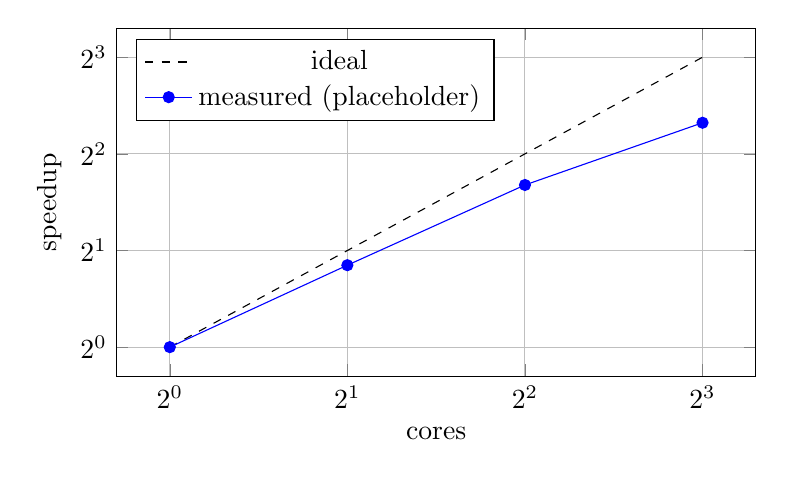
\begin{tikzpicture}
	\begin{axis}[width=0.8\textwidth,height=6cm,xlabel={cores},ylabel={speedup},xmode=log,ymode=log,log basis x=2,log basis y=2,legend pos=north west,grid=both]
      \addplot[dashed] coordinates {(1,1)(2,2)(4,4)(8,8)};
      \addplot[mark=*,blue] coordinates {(1,1)(2,1.8)(4,3.2)(8,5.0)};
      \legend{ideal,measured (placeholder)}
    \end{axis}
  \end{tikzpicture}
  \caption{Strong scaling speedup.\TODO{THIS IS TOTALLY PLACEHOLDER LOL}}
\end{figure}

\subsection{Effect of the design choices}
\begin{itemize}
\item \texttt{-p mom} vs.\ \texttt{-p rand}: rounds, time per round, total time.
\item Rebalancing: random vs.\ sorted/reverse data, with and without \texttt{-r}; elements moved, imbalance per round.
\item Switch size (\texttt{-s}) sweep.
\item Pure MPI vs.\ hybrid at equal core count.
\item In-memory generation (\texttt{-g}) vs.\ file read: time to load. \TODO{Ce ne freca? sarebbe solo un workaraound alla poca memoria}
\end{itemize}

\subsection{Discussion}
\TODO{Comparare con il modello in \cref{sec:design}; spiegare come e perché lo scaling si appiattisce; cita~\cite{amdahl} e~\cite{gustafson}. Confrontare con baseline sequenziale.}

\section{Evaluation and significance of results}\label{sec:eval}
\TODO{Boh una sorta di conslusione sui risultati ottenuti, se suono buoni, scarsi, or whatever}

\section{Conclusions}
\TODO{Boh ci possono essere migliaia di cose da fare, piazzamento NUMA-aware, GPU offload, $k$ quantili.}

\section{AI usage statement}
\TODO{Let's see what to write exactly.}

\begin{thebibliography}{99}
\bibitem{phillips} Phillips, \emph{Parallel Selection}, lecture notes (S14). \TODO{Altri dettagli?}
\bibitem{blum} M.~Blum, R.~W.~Floyd, V.~Pratt, R.~L.~Rivest, R.~E.~Tarjan, ``Time bounds for selection'', \emph{J.\ Computer and System Sciences} 7(4):448--461, 1973.
\bibitem{hoare} C.~A.~R.~Hoare, ``Algorithm 65: Find'', \emph{Communications of the ACM} 4(7):321--322, 1961.
\bibitem{floydrivest} R.~W.~Floyd, R.~L.~Rivest, ``Expected time bounds for selection'', \emph{Communications of the ACM} 18(3):165--172, 1975.
\bibitem{saukas} E.~L.~G.~Saukas, S.~W.~Song, ``A note on parallel selection on coarse-grained multicomputers'', \emph{Algorithmica} 24:371--380, 1999.
\bibitem{bader} D.~A.~Bader, J.~J\'aJ\'a, ``Practical parallel algorithms for dynamic data redistribution, median finding, and selection'', \emph{J.\ Parallel and Distributed Computing} 58:238--254, 1999.
\bibitem{splitmix} G.~L.~Steele Jr., D.~Lea, C.~H.~Flood, ``Fast splittable pseudorandom number generators'', \emph{OOPSLA}, 2014.
\bibitem{amdahl} G.~M.~Amdahl, ``Validity of the single processor approach to achieving lare scale computing capabilities'', \emph{AFIPS Spring Joint Computer Conference}, 1967.
\bibitem{gustafson} J.~L.~Gustafson, ``Reevaluating Amdahl's law'', \emph{Communications of the ACM} 31(5):532-533, 1988.
\bibitem{mpi} Message Passing Interface Forum, \emph{MPI: A Message-Passing Interface Standard}. \TODO{Versione e url?}
\bibitem{openmp} OpenMP Architecture Review Board, \emph{OpenMP Application Programming Interface}. \TODO{version and url}
\end{thebibliography}

\end{document}
